\documentclass[12pt]{article}
\usepackage{xeCJK}
\usepackage{amssymb,tikz,pdftexcmds,xparse}
\usepackage{url}
\usepackage{titlesec}

\usepackage{indentfirst}
\usepackage{amsmath}
\usepackage{enumitem}
\usepackage{xcolor}
\usepackage{algorithm}
\usepackage{algorithmic}
\usepackage{graphicx}   % for trimming images
\usepackage{tikz}
\usetikzlibrary{shapes, arrows.meta, positioning}

% % Answer: [trim={left bottom right top},clip]
% % Ex. 1: trim from left edge
% \includegraphics[trim={5cm 0 0 0},clip]{example-image-a}
% % Ex. 2: trim from right edge
% \includegraphics[trim={0 0 5cm 0},clip]{example-image-a}

% Use the trim option, which takes four space separated values.

%  trim={<left> <lower> <right> <upper>}



% Adjust spacing for section
\titlespacing*{\section}
{0pt} % Left spacing
{10pt} % Spacing before the section
{4pt}  % Spacing after the section

% Adjust spacing for subsection
\titlespacing*{\subsection}
{0pt} % Left spacing
{8pt} % Spacing before the subsection
{3pt}  % Spacing after the subsection

% Adjust spacing for subsubsection
\titlespacing*{\subsubsection}
{0pt} % Left spacing
{12pt} % Spacing before the subsubsection
{1pt}  % Spacing after the subsubsection


\tikzset{box/.style={
    minimum size=0.225cm,
    inner sep=0pt,
    draw,
  },  
  insert mark/.style={
    append after command={%
         node[inner sep=0pt,#1]
           at (\tikzlastnode.center){$\checkmark$}
     }     
  },
  insert bad mark/.style={
    append after command={%
         [shorten <=\pgflinewidth,shorten >=\pgflinewidth]
         (\tikzlastnode.north west)edge[#1](\tikzlastnode.south east)
         (\tikzlastnode.south west)edge[#1](\tikzlastnode.north east)
     }     
  },
}

\makeatletter
\NewDocumentCommand{\tikzcheckmark}{O{} m}{%
  \ifnum\pdf@strcmp{#2}{mark}=\z@%
    \tikz[baseline=-0.5ex]\node[box,insert mark={#1},#1]{};%
  \fi%
  \ifnum\pdf@strcmp{#2}{bad mark}=\z@%
    \tikz[baseline=-0.5ex]\node[box,insert bad mark={#1},#1]{};%
  \fi%
  \ifnum\pdf@strcmp{#2}{no mark}=\z@%
    \tikz[baseline=-0.5ex]\node[box,#1]{};%
  \fi%
}
\makeatother


% Redefining maketitle
\makeatletter
\renewcommand{\maketitle}{
  % \begin{center}
    {\LARGE \@title \par}      % Title in large font
    % \vspace{2mm}               % Space between title and author
    % {\large \@subtitle \par}      % Subtitle in large (but smaller than title) font
    % \vspace{2mm}               % Space between title and author
    {\large \@author \par}     % Author in large (but smaller than title) font
    % Date is removed, so no command for date here
  % \end{center}
  % \vspace{5mm}                 % Space after the title block
}
\makeatother

% Language setting
% Replace `english' with e.g. `spanish' to change the document language
\usepackage[english]{babel}

% Set page size and margins
% Replace `letterpaper' with `a4paper' for UK/EU standard size
\usepackage[letterpaper,top=2cm,bottom=2cm,left=2cm,right=2cm,marginparwidth=1.75cm]{geometry}

% Useful packages
\usepackage{amsmath}
\usepackage{graphicx}
\usepackage[colorlinks=true, allcolors=blue]{hyperref}
\usepackage{listings}
\usepackage{color}
\usepackage{minted}

% https://www.overleaf.com/learn/latex/Positioning_images_and_tables#Basic_positioning
% To position the image to the centre
\usepackage[export]{adjustbox}  

\usepackage{xcolor}
\usepackage{xparse}
\usepackage{blindtext}
\usepackage{hyperref}   % For hyperlinks

\usemintedstyle{manni}

\NewDocumentCommand{\codeword}{v}{%
% \texttt{\textcolor{blue}{#1}}%
\texttt{\textcolor{black}{#1}}%
% \mint{html}|v|%
}

% \newcommand{\img_folder}{presentation-img_0065-scale_0_5-best_lambda_0_03-kernel_512-model_img_0065-scale_0_5-kernel_512-sigma_0_3-T_128_2024_05_26_09_38_07_epoch_9774-trained_on_img_0065}

% \lstset{language=C,keywordstyle={\bfseries \color{blue}}}

\definecolor{dkgreen}{rgb}{0,0.6,0}
\definecolor{gray}{rgb}{0.5,0.5,0.5}
\definecolor{mauve}{rgb}{0.58,0,0.82}

\lstset{frame=tb,
  % language=Java,
  language=Python,
  aboveskip=3mm,
  belowskip=3mm,
  showstringspaces=false,
  columns=flexible,
  basicstyle={\small\ttfamily},
  numbers=none,
  numberstyle=\tiny\color{gray},
  keywordstyle=\color{blue},
  commentstyle=\color{dkgreen},
  stringstyle=\color{mauve},
  breaklines=true,
  breakatwhitespace=true,
  tabsize=2
}

\title{MTH786P Project - Diabetes Prediction}
\author{Thanh Trung Vu - 230849442}

\usepackage[utf8]{inputenc}
\usepackage[english]{babel}
\usepackage{biblatex}
\addbibresource{references.bib}

\begin{document}

\setlength\parskip{0.5em plus 0.1em minus 0.2em}

% \vspace{-30pt}


% \begin{figure}
%     \centering
%     
\includegraphics[width=0.3\linewidth]{images/QMUL logo.png}
%     % \caption{Enter Caption}
%     % \label{fig:enter-label}
% \end{figure}

% \vspace{-30pt}

% \maketitle

{\large \textbf{MTH767P Neural Networks and Deep Learning Mini Project - CNN and UNET in Image Reconstruction}}

{\large \textbf{Thanh Trung Vu - 230849442}}

% \vspace{-12pt}

\section{TASK}

\begin{center}
% \begin{figure}
    % \centering
    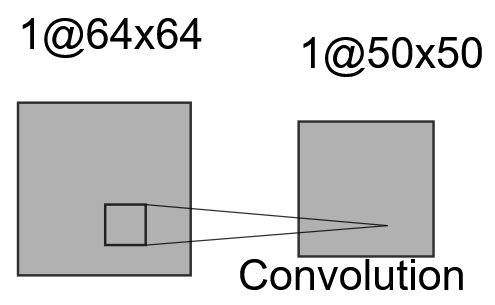
\includegraphics[width=0.3\linewidth]{cnn_example_1.png}
    
    \caption{CNN Example}
    \label{fig:cnn_example_1}
% \end{figure}
\end{center}

We have seen a fully connected layer. In essence, a convolutional layer differs from a fully connected layer in the way we think about the connection between two consecutive layers. Instead of a weight matrix, we have a filter. In the 1D case, we can image have a vector of weights and "slide" it across the input vector. In the 2D case, we can treat each layer as a 2D matrix instead of a vector, and the filter as a small square that "slides" across the input matrix. For this project, since we are doing an image processing task, we will assume convolution means 2D convolution. At each position we have the normal dot product operation with the filter and the subset of the input to create one value in the output. Some help visualisations can be found at \cite{cnn_vis}.
We can also have more than one filter in each layer. The number of filters is also called the number of channels, since each filter produces a new matrix.
% Note that a convolution is equivalent to a normal 
% A normal fully connected layer can also be seen as a convolutional layer where each filter is the whole row of the weight matrix.
The idea is that this feature map that highlights a specific feature that the filter is designed to detect.

%%%%%%%%%% BEGIN CONVOLUTION ANALOGY
% A convolution operation is equivalent to a normal fully connected layer.
It can be helpful to 
make an analogy of
% relate 
a convolution as a normal matrix multiplication operation.
For example, imagine 2 consecutive layers with vectors $x_1$ and $x_2$, where $d_1 = 81$ and $d_2 = 49$. The weight matrix $W_1$ will have $81 \times 49 = 3969$ values.

However, let's say we treat $x_1$ as a $9 \times 9$ matrix and $x_2$ as a $7 \times 7$ matrix. And let's say that each value in $x_2$ is a linear combination of $9$ values on $x_1$. Then $W_1$ will have only $9 \times 7 \times 7 = 441$ non-zero values.

Furthermore, let's say that each combination have the same set of 9 weights, and $(x_2)_{i,j}$ comes from $(x_1)_{p,q}$ for $p = i, ..., i+2$, $q = j, ..., j+2$. The weight matrix $W_1$ will still have $441$ non-zero values but actually we can just store the 9 unique values.

We can represent this as a convolution operation with a $3 \times 3$ filter, i.e. the matrix with those 9 unique values. The filter will move across the matrix $x_1$ and produces $x_2$. 
%%%%%%%%%% END CONVOLUTION ANALOGY

The output after applying one filter can be called a feature map.

If we have more than 1 filters, we can have more feature maps.

A reasoning behind this scheme is that each filter extracts a different type of feature. For example


% % Sobel Operator for Edge Detection
% The Sobel operator for edge detection consists of two 3x3 filters, one for detecting edges in the horizontal direction and one for the vertical direction.

% % Horizontal Edge Detection Filter (Gx)
% The horizontal edge detection filter \(G_x\) is given by:

this filter 

\[
G_x = \begin{bmatrix}
-1 & 0 & 1 \\
-2 & 0 & 2 \\
-1 & 0 & 1
\end{bmatrix}
\]

can detect a horizontal edge, while this filter

% % Vertical Edge Detection Filter (Gy)
% The vertical edge detection filter \(G_y\) is given by:

\[
G_y = \begin{bmatrix}
-1 & -2 & -1 \\
0 & 0 & 0 \\
1 & 2 & 1
\end{bmatrix}
\]

can detect a vertical edge.

% % Explanation
% In these filters, the central element corresponds to the pixel being evaluated, and the surrounding elements correspond to the neighboring pixels. The convolution of these filters with an image highlights regions of high intensity change, which correspond to edges.

In addition to a normal convolutional layer, we can also have a pooling layer, usually a max-pooling layer where each filter now outputs the maximum value in each region, 
% or an average-pooling layer (essentially a normal convolution layer with a filter having only 1's), 
rather than the matrix multiplication. The goal is to select the most significant value from a local region of the feature map.


We can hope that, as we increase the number of filters and let the network learn the parameters of the filters, we can obtain meaningful filters, each of which can extract a useful feature. While the idea of obtaining useful features exists in all neural network architectures, the idea of using filters in convolutional neural networks is highly compartible with image data which can be represented as 2D matrices.

CNN has been shown to work very well in learning relevant features from image data. In fact, since each layer is still a series of matrices, we can visualise each layer to have an idea of the features which the network is learning.

If we compare a convolutional layer to the equivalent version of a fully connected layer, then we can see that it is more efficient: there are fewer unique values to store and fewer calculations to produce the same output. A difference is that, when backpropagation is performed, in the fully-connected version, each parameter is updated separately, so the number of unique values can increase. On the other hand, in convolutional layer, back propagation is carried out in a more restricted way so that only the unique values are updated. More information on back propagation in CNN: \url{https://deeplearning.cs.cmu.edu/F21/document/recitation/Recitation5/CNN_Backprop_Recitation_5_F21.pdf}. This means that the concept of filters stays, and each filter will represent a feature-extractor, (rather than just a massive transformation). 

As Le-Cunn and colleagues discovered in 1989, CNN is particularly helpful in computer vision tasks, one of which was to recognise hand-written letters and digits.




\newpage




\printbibliography


The following list contain the primary Python libraries used in the implementation of this project.

\vspace{-6pt}

\begin{itemize}
\setlength\itemsep{-0.3em}
  % \item \codeword{NumPy} : for numerical representations and operations, including vector and matrix multiplication.
  \item \codeword{PyTorch} : 
  \item \codeword{matplotlib} and \codeword{seaborn} : for data visualisation, including the creation of histograms and box plots.
  \item \codeword{pandas} : for data analysis and manipulation tasks, such as value replacement.
  \item \codeword{scikit-learn} : for comparisons with other learning algorithms.
  \item \codeword{random} : for generating random numbers, particularly in K-fold cross-validation and bootstrap sampling.
  \item \codeword{wandb} : for logging
\end{itemize}

\end{document}